\chapter{Introduction}

Financial institutions make decisions to buy or sell assets for many reasons, including: customer requests, fundamental analysis\cite{fundamental-analysis}, technical analysis\cite{technical-analysis}, top-down investing\cite{td-investing}, and bottom-up investing\cite{bu-investing}.
High-level trading strategies oftentimes define how an institution positions itself in financial markets and, if applicable, towards its customers.
Regardless of the high-level trading strategy that is being applied, the invariable outcome is a decision to buy or sell assets.
This work aims to take a step towards answering the important question of how one can optimize a purchase or sale of an asset on a stock exchange with the use of reinforcement learning techniques.
The subsequent sections will elaborate this problem briefly and state the research objectives of this work.
We will list the contributions made to research communities throughout this work, followed by a brief overview of the structure of this report.

\section{Context and Problem Statement}
\label{sec:problem-statement}

We are concerned about the way assets, specifically \textit{securities} (exchange traded assets), are traded on stock exchanges.
There is little consensus as to when corporate stock was first traded; some argue that the exchange, in the form we know it today, dates back as far as 1531, when East Indian Company stock was traded in Antwerp\cite{stock-exchange}.
Modern financial markets such as the London Stock exchange (LSE), the New York Stock Exchange (NYSE), but also the numerous crypto-currency exchanges which have appeared suddenly in the last few years, all rely on the very same principles as back then.
They allow participants (called "traders") to buy or sell a given amount of a security at a particular price.
In the late 1990s, the regulatory authorities started to let traders access the markets using electronic communications networks (ECNs) and so a new era dawned \cite{patterson2012dark}.
Since then, high frequency trading (HFT) and sophisticated algorithmic trading vehicles have made up a substantial and ever-increasing part of electronic market participants.
Their servers are oftentimes located within exchanges and specialized computer networks have been constructed to provide millisecond-level advantage in the arbitrage of trades between exchanges.
Ever since, traders without such equipment and techniques have felt that they are at a disadvantage in such an environment. \cite{patterson2012dark}
While anything except trading through electronic channels would be unthinkable today, a certain gap still exists between trading companies that have fibre access to the exchanges or supporting algorithms and investors who do not.
As a result, investors are forced to take an initial loss into account when buying or selling securities, which they might not even be aware of.
In order to understand why these losses are incurred, we have to have a basic understanding of a so-called order book and how securities are bought at an exchange.

\begin{figure}[H]
    \centering
    \makebox[\linewidth]{
        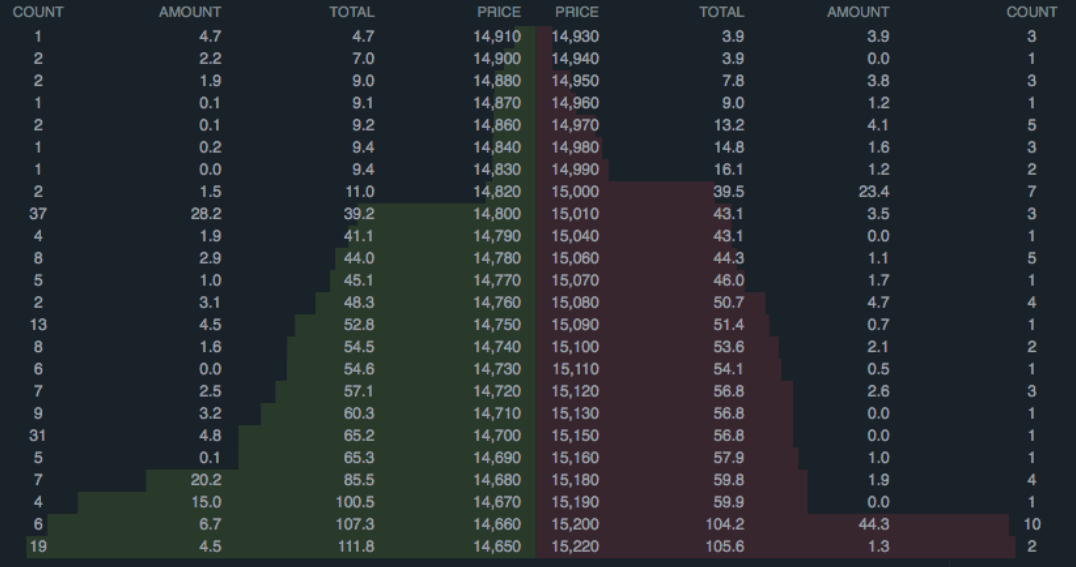
\includegraphics[width=12cm]{orderbook-gdax.png}
    }
    \caption{Order book snapshot: https://www.bitfinex.com/t/BTC:USD}
    \label{fig:intro-orderbook}
\end{figure}

Figure \ref{fig:intro-orderbook} shows a snapshot taken at some time $t$ of the trading pair Bitcoin (BTC) versus US dollar (USD) taken on the Bitfinex\footnote{https://www.bitfinex.com} cryptocurrency exchange.
The order book shows two columns, the parties who are willing to buy are on the left and the parties who are willing to sell are on the right.
The two columns indicate the number of buyers and sellers (\textit{count}) who are willing respectively to buy and sell a certain \textit{amount} for a given \textit{price}.
The column \textit{total} is the cumulative sum of the amount, or volume, on each side.
The difference between the figures in each column is the \textit{spread}.
In this particular case, the current best \textit{bid} price--at which someone is willing to buy--is \$14,910.00 and the best ask-price at which someone is willing to sell, is \$14,930.00.
Therefore, the spread is currently \$20.00.
\\
\\
Suppose we want to buy 1.0 BTC.
Two possible ways to do so are:
\begin{enumerate}
    \item Buy 1.0 shares right away for \$14,930.00 from a seller. To do so, we submit a \textit{market} order.
    \item State a price at which we are willing to buy 1.0 shares at price $p$, for example at \$14,910.00, and wait until someone is willing to sell at this price. To do so, we submit a \textit{limit} order.
\end{enumerate}

Both types of orders come with their advantages and disadvantages.
A market order ensures that we will be able to acquire the stated amount of shares immediately for \$14'930.00, provided that no one else  has a prior claim to them and that the seller does not cancel his/her listing.
In this case, we are automatically willing to pay the next available best price.
However, we do pay a premium compared to the limit order since ask prices are listed higher than bid prices and the more shares one wants to buy, the more sellers we have to contact and accept their offers at an increased price.
With a limit order, the exchange guarantees that we will pay \$14,910.00 or less.
That is, when a seller is willing to sell for the stated price or less, the exchange will match the offers of both parties.
However, this comes with the risk that we will never be able to buy if nobody is going to sell at the demanded price, and this will force us to buy the shares demanded at a later point in time.
As the price of a share evolves over time, we might get lucky and be able to buy at a cheaper price than at the time of the initial attempt.
The other scenario is that the price did not develop in our favour such that we have to buy at a higher price later on; thus, we pay a so-called \textit{opportunity cost}.
A third order type, the \textit{cancel} order, allows a trader to cancel his/her previously posted limit or market order at any given point in time.
%Ultimately, we have a brief understanding of what traders are allowed to do at a stock exchange.
%We will now elaborate briefly how such a relatively simple concept of an order book and three types of orders can lead to a diverse range of situations a trader can find himself whereas at times this may be beneficial for his intentions and at times it will lead to paying a premium.
%If a seller realizes that we are about to buy for price $p$ at which is was willing to sell, he then could \textit{cancel} his offer as his incentive is to sell for a higher price.
%Perhaps this has been his/her intention to only post an offer but withdrawal as soon as a counter-offer will be listed that is close to his/her price.
%This method is known as \textit{quote stuffing}.

With this brief understanding of how traders can interact with the exchange, we can define the problem of \textit{order placement} as follows.
Order placement determines the price at which a trader places its order.
The aim of optimizing order placement are to minimize the opportunity cost and, ideally, achieve a more favorable price payable (or receive) than what is currently being offered at the market price.
Literature therefore specifies a time scale of from ten to one hundred seconds within which a trader has to complete his task of either buying or selling the shares \cite{guo2013optimal}.
A time scale of less than ten seconds applies in high frequency trading and one of above 100 seconds is known as \textit{order execution optimization}.
Thus, could we define order placement optimization as the price $p$ at which one should attempt to buy or sell $i$ shares within a time horizon $H$ of 100 seconds?
As we shall see, optimizing placement is not as trivial as one might think, even though the concepts of the order book and the three order types a trader can choose from are admittedly simple.
There are various properties in a limit order book, as well as the behaviour of the market participants, that changes over time.
All of which can drastically interfere with the intention of buying and selling.
Furthermore, since the foundation of electronic trading networks and algorithmic trading, the amount and sophistication of other market participants has been ever-increasing, with everyone aiming for an advantage over others.
%However, the prices for some financial products, including crypto-currencies, are very volatile such that it is likely to be able to buy for less than what is offered at the mentioned time $t$.
%In addition, there might be buyers and sellers in the near future which would consume our order.
%Thus, placing orders \textit{deeper} in the book and wait could be beneficial.
%
%According to Guo et. al. \cite{guo2013optimal} algorithmic trading is based on two different time scales: \textit{order execution} concerns about optimally slicing big orders into smaller ones in order to minimize the \textit{price impact}, that is, on a daily or weekly basis.
%\textit{Order placement} on the other hand concerns about optimally placing orders within ten to hundred seconds.
%In this thesis we are concerned about the latter, which conforms the context of the problem:

The fact that reinforcement learning functions by maximizing rewards makes this technique unarguably suitable in this context.
That is, how to place orders according to the given market condition and therefore protect an investor form paying the aforementioned premium to other participants in the market.
Ideally, such a learner will be able to foresee short term trend changes such that the investor ultimately benefits from a better price at which to buy or sell the asset. 

\section{Research objectives}

This work extends the findings of Kearns et. al. who have studied the behavior of order placement and order execution\cite{nevmyvaka2005electronic}, and further developed a reinforcement learning strategy\cite{nevmyvaka2006reinforcement} in order to proceed optimization.
Their work has pre-processed and applied features, which were derived from order book data, to a reinforcement learning algorithm which is similar to Q-Learning.
Rather than constructing features by hand, the work in this thesis makes an attempt to benefit from hidden patterns in raw market data by using deep reinforcement learning techniques.
In addition, the crypto-currency domain is chosen, instead of traditional stocks.
Furthermore, while the previously mentioned work of Kearns et al. had success in using pre-processed market data as features, we believe that raw market data in combination with deep reinforcement learning can be equally successful.
Hence, our ambition is to determine if deep reinforcement learning is perhaps an even more suitable choice in order to deal with unexpected market situations.

The research proceeded and presented with this thesis is as follows.
To simulate and understand the outcome of order placement and more importantly build a reinforcement learning environment that allows interaction with agents, we are required to build a framework.
The framework should provide collection and market data processing capabilities in order to reproduce a historical order book that serves as a data source.
Further, we require that the framework provides the functionality of a match engine which emulates the functionality of a stock exchange that can match orders and determine the resulting price paid (or received) according to the historical order book.
Ultimately, a reinforcement learning environment should be built which allows to simulate and evaluate order placement.
The environment should allow direct user interaction, in order to place orders on demand, and interaction with agents which act as intelligent traders.
However, the first use of the environment will be to simulate the behaviour of order placement in a historical USD/BTC market and try to find properties which may be beneficial for optimization with deep reinforcement learning.
With this knowledge, we then build two reinforcement learners whereas both act as an intelligent trader and place limit orders that provide an incentive to buy or sell an asset at a favorable price.
Both agents are driven by an end-to-end learning process by which the agent improves based on the outcome of the placed orders and ultimately learns a strategy that allows to buy and sell shares at favorable prices.
The former agent is an adaption of the well known Q-Learning algorithm and optimizes based on the amount of assets to buy or sell and a given time horizon only.
The latter is a deep reinforcement learning agent that makes use of a convolutional neural network in order to detect patterns in market data.
Therefore, we have to determine how to shape the data such that an agent can detect patterns which allow to learn how to place orders at the most optimal price.
Finally, the main objective of this research can be formulated in one sentence:
\begin{quote}
    How should one design a deep reinforcement learning environment and construct features, which are derived from a limit order book, such that an agent can detect patterns to mitigate the impact of the important problem of limit order placement?
\end{quote}
Clearly, included in the study are the limitations of this setup that we have considered here.

\section{Contributions}

This thesis makes use of concepts from various research communities in order to work towards the above mentioned objectives.
The particular contributions made throughout the project are:
\begin{itemize}
    \item Information retrieval techniques are applied in order to collect and process financial data sets.
    We analyze the data and find patterns which might be beneficial for the process of limit order placement optimization.
    Feature sets are then constructed which incorporate the found patterns and allow deep reinforcement learning agents to learn an order placement strategy.
    \item We study how to translate the problem of limit order placement into a reinforcement learning context.
    With the use of software engineering techniques we then build an environment which simulates a rudimentary stock exchange and allows an agent to optimize on the given problem.
    Therefore we make use of the OpenAI Gym\footnote{https://github.com/openai/gym} library and contribute our work to the community to proceed further investigations.
    \item Investigations of reinforcement learning agents applied to the process of \textit{order placement} (and the closely related process known as \textit{market making}) will unveil the capabilities of deep reinforcement learning on a continuously changing state space derived from a multivariate time series.
    Under these circumstances we determine the possible benefits and limitations of deep reinforcement learning, when applied to noisy environments.
\end{itemize}

\section{Document structure}

In Chapter \ref{chap:preliminaries} we first provide background information to the reader concerning the components of a stock exchange and the fundamentals of the closely related time series.
We further make the reader familiar with (Deep) Reinforcement Learning.
In Chapter \ref{chap:related-work} we elaborate on the behaviour of order execution followed by approaches of both statistical and machine learning nature.
Chapter \ref{chap:data} explains the process of data collection and its preparation which was done prior its use in the following chapters.
Namely, Chapter \ref{chap:setup} explains the experimental setup of the Reinforcement Learning environments, the agents and the features being processed and used.
In Chapter \ref{chap:analysis} we then analyze the data and proceed execution placement with various techniques, including the reasoning of our findings.
Finally, Chapter \ref{chap:conclusion} formulates a conclusion of our findings and states a future research direction.
